\documentclass[10pt,a4paper]{article}
\usepackage[utf8]{inputenc}
\usepackage{amsmath}
\usepackage{amsfonts}
\usepackage{amssymb}
\usepackage[margin=3cm]{geometry}
\usepackage{xspace}
\usepackage{enumerate}
\usepackage{graphicx}
%\fontfamily{garamond}
%\selectfont
\begin{document}

\newcommand{\ether}{Ether\xspace}
\newcommand{\ie}{{i.e.}\xspace}
\newcommand{\eg}{{e.g.}\xspace}

\newcommand{\parameterize}[1]{{\ensuremath{#1}}\xspace}
\newcommand{\R}{\parameterize{R}}
\newcommand{\N}{\parameterize{N}}
\newcommand{\T}{\parameterize{T}}
\newcommand{\x}{\parameterize{\mathbf x}}
\newcommand{\udd}{\parameterize{\ddot{u}}}
\newcommand{\U}{\parameterize{\ddot{U}}}
\newcommand{\NC}{\parameterize{N^C}}

\renewcommand{\labelitemi}{$\cdot$}

\begin{center}
{\LARGE\bf Some Basic Analysis of the Ethereum Platform}

Aeron Buchanan, Version 1
\end{center} 

\vspace*{-.6cm}
\section*{Intro}

I'm going to start at the beginning and describe everything. This is important for exposing bad assumptions or simplifications. Please bear with me.

Ethereum is a de-centralized collaborative shared-state update platform with a turing-complete processing capability. It is rather like a shared cloud computer the size of the internet:

\begin{center}
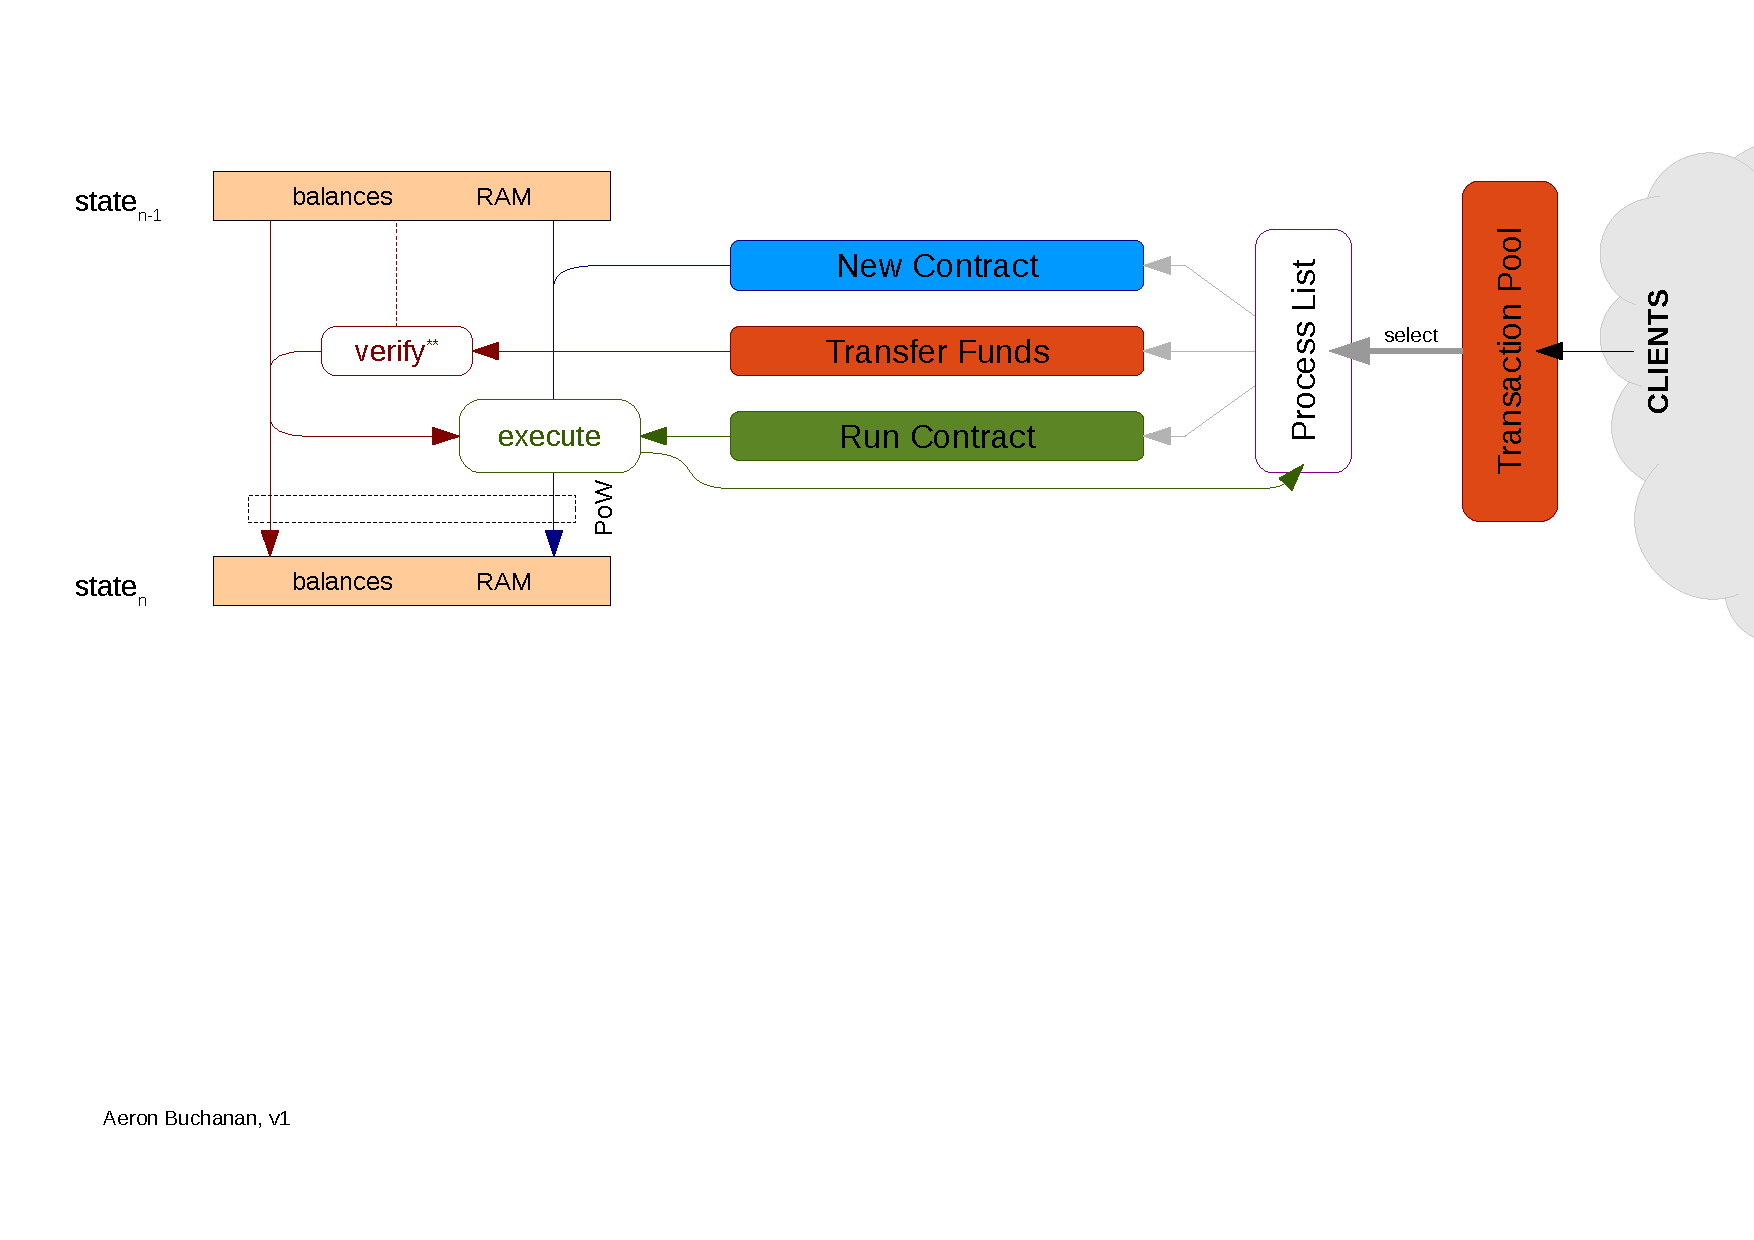
\includegraphics[trim=0cm 10cm 0cm 2cm, clip, width=15cm]{FlowDiagramEthereumOnly.pdf}
\end{center}

Anyone can initiate a transaction to send {\tt [funds + data]} to another account, as long as they have sufficient funds available. That transaction will either 

\begin{enumerate}[\hspace{1cm}1.] \itemsep=0pt
\item create a new contract using the {\tt funds} and {\tt data}, or 
\item transfer funds to another account
\end{enumerate} 
 
The target account for {\tt fund} transfers can either be
 
\begin{enumerate}[\hspace{1cm}a)] \itemsep=0pt
\item a contract account (i.e. execute that contract, using the {\tt data}), or
\item another normal account (just transfer {\tt funds}; ignore the {\tt data})
\end{enumerate}
 
A contract can update its own RAM arbitrarily and generate new transactions to do any of the above with its own funds.

\begin{center}
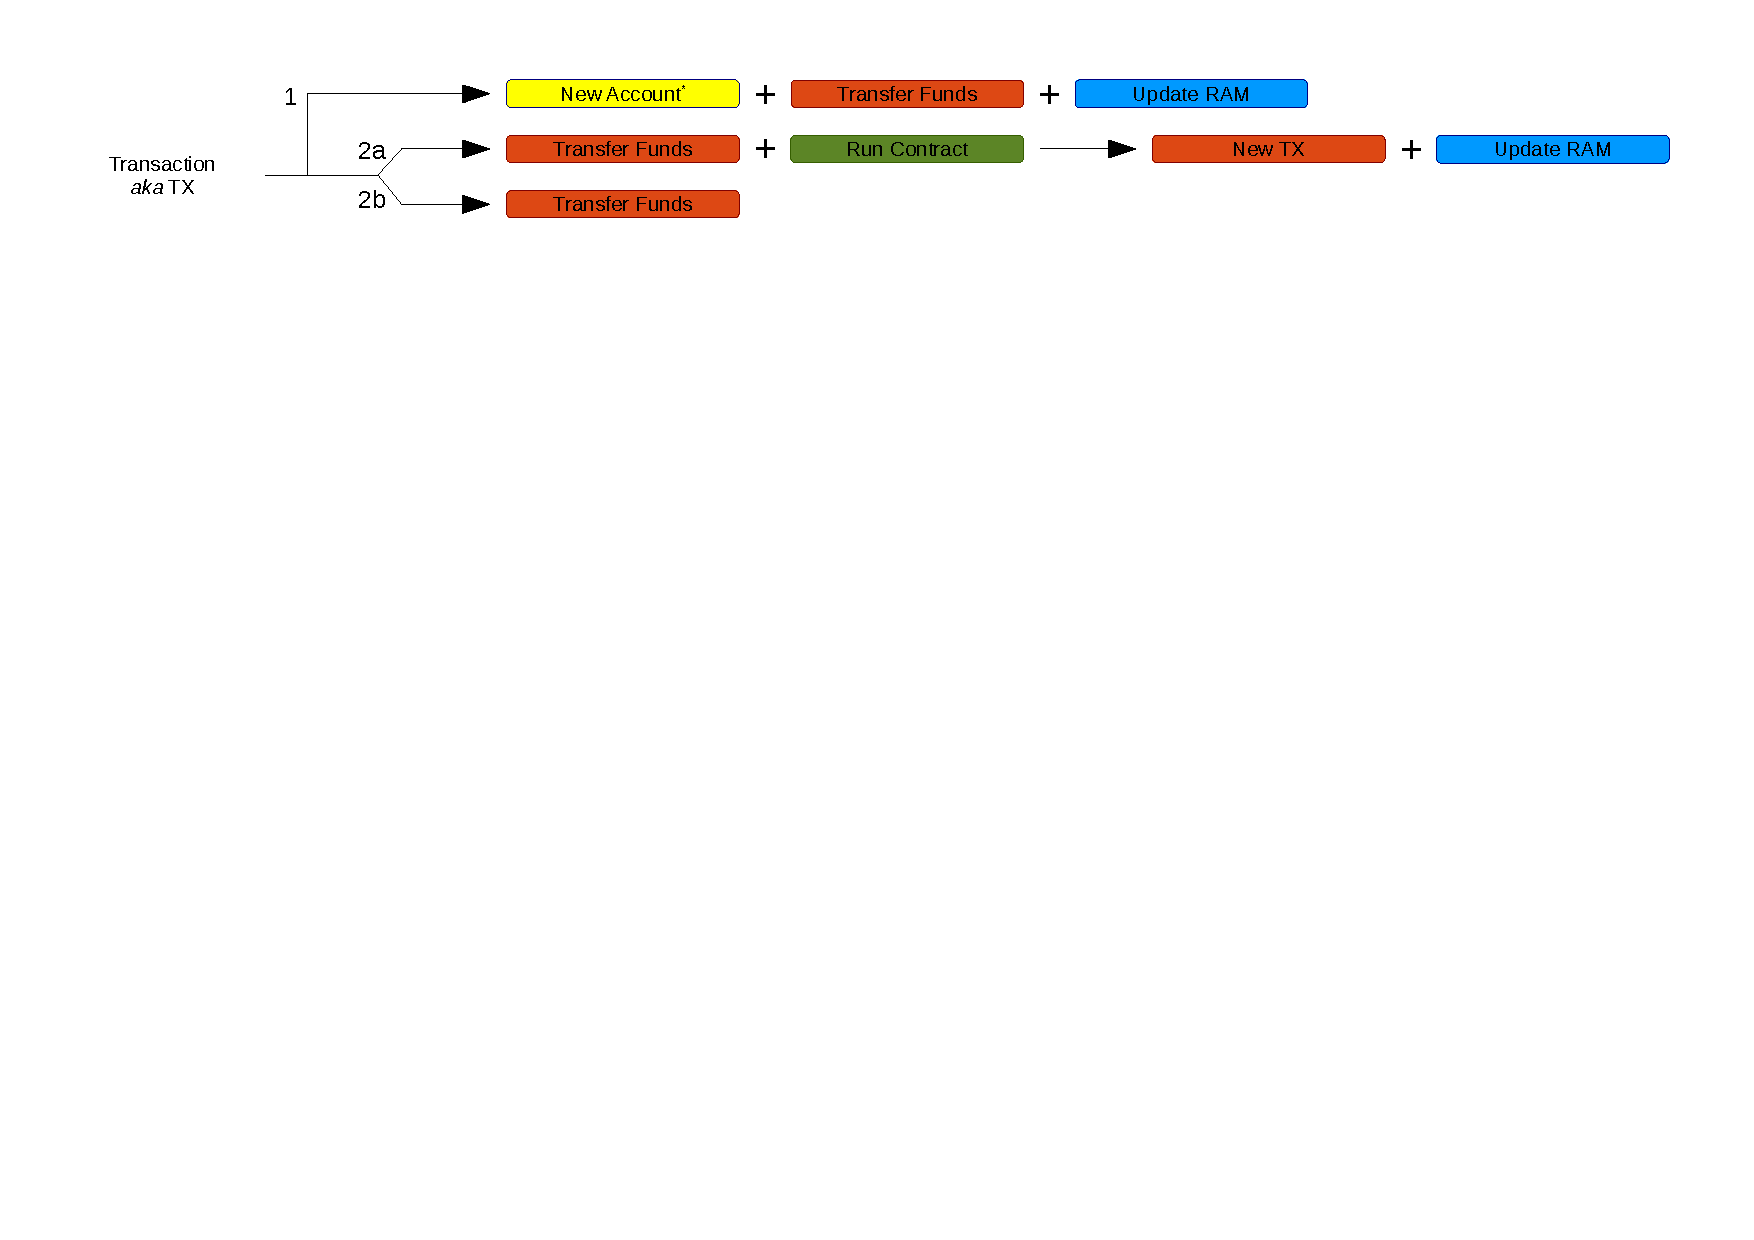
\includegraphics[trim=1cm 17cm 1cm 1cm, clip, width=15cm]{FlowDiagramEthereumTXTypes.pdf}
\end{center}

Note: beyond a free quota of operations, every executed instruction must be paid for from the contract's balance.

Ethereum is realized by a network of computer processing entities, or nodes, that are each independently calculating the state progression, and then reaching a consensus to agree on the "true" state. By way of implementation, information about any given state update is held in something called a block. Nodes select transaction requests posted by anyone with an Ethereum account and calculate the resulting block to add to the chain of blocks that represents the entire state history of Ethereum. As all nodes do this independently, we let the node who (correctly) does this first have the definitive say as to what the next update is, \ie which transactions are included as part of the next state progression. There is a payment of newly created ether, \R for getting there first (as a way of reward for participating) and, importantly, the potential to receive compensation for performing all the necessary verifications and execution of computation, via transaction and computation fees. Additionally, a proof-of-work (PoW) calculation (computation that is essentially wasted) is required to prove the time of completion is as stated. The PoW has the side-effect that, if no-one included any transactions in the block they are racing to add and all the nodes were of equal computational power, it would be random as to who won each time, \ie with \N nodes the chance of any node getting their block onto the block chain is $\frac{1}{\N}$. If the distribution of computing power is uneven, the chance is in proportion to the fraction of the total network's compute power that a particular node has, \eg a node with 25\% of the compute power of the total network has a 25\% chance of getting any of their block updates onto the consensus block chain. Because of the rewards available, nodes are referred to as miners. To go some way to reward miners who only just missed out on getting their block onto the chain, a GHOST reward is paid to them.

\subsection*{\ether Flow}

Looking at the flow of \ether in Ethereum, we can categorize the things that are responsible for \ether moving around:
\begin{itemize} \itemsep=0pt
\item The System, which creates \ether to reward successful miners
\item miners, who undertake the PoW and perform the Ethereum computation 
\item buyers, who pay for Ethereum computation to be performed
\item simples, who give their \ether away in basic transactions
\item savers, who hold on to their \ether
\item black holes, where lost \ether goes after pouring Dr Pepper into the only computer that can access your wallet, etc
\end{itemize}
and it could be that an actual real participant combines several of these personalities. Because I think in diagrams, here's a picture:

\begin{center}
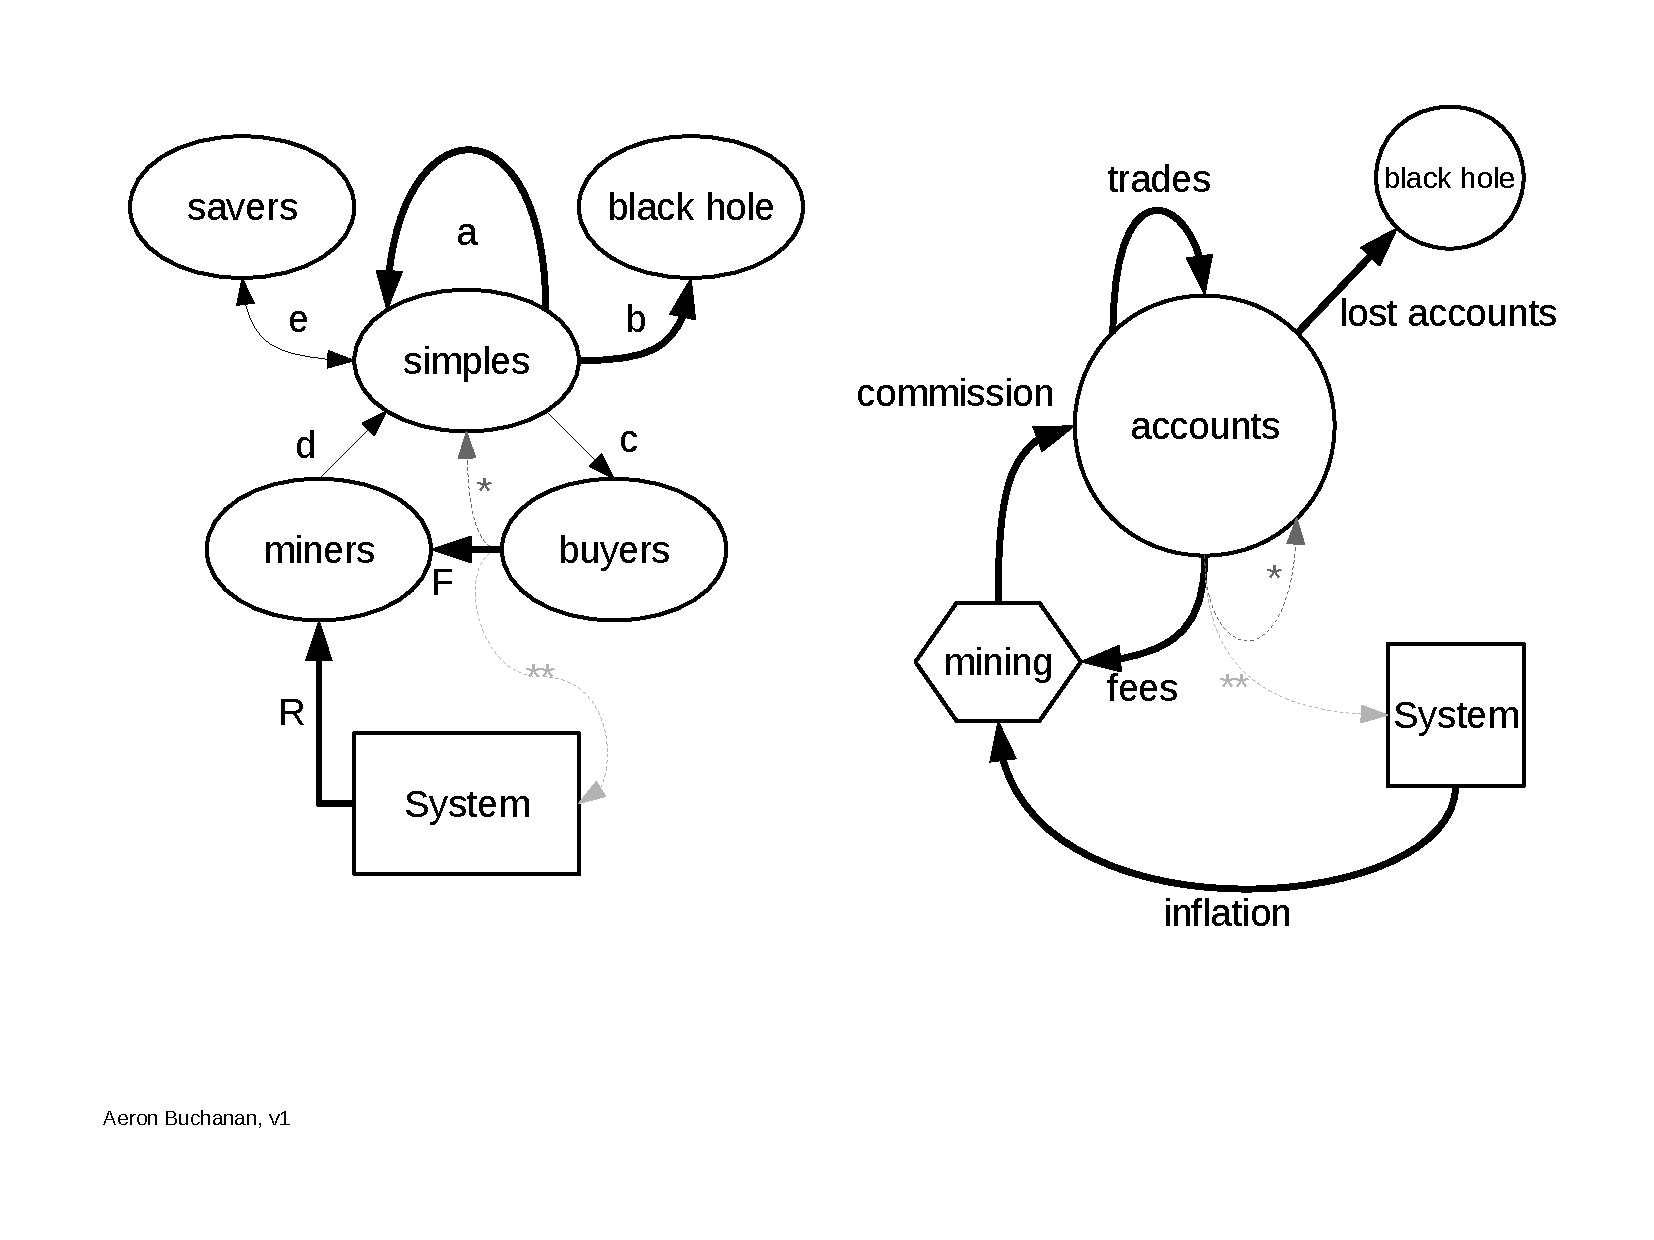
\includegraphics[trim=1cm 4cm 1cm 1.5cm, clip, width=15cm]{EtherFlow.pdf}
\end{center}

The two are equivalent. The thick arrows are the descriptions of the above processes and the thin ones are extra to account for real participants being combinations. A few comments:
\begin{enumerate}[\hspace{1cm}] \itemsep=0pt
\item trades: I'm going to ignore basic trades as that will probably just look like bitcoin. 
\item lost accounts: as long as $b\ \not\!\gg \R$, we're OK.
\item commission: $d = \R + F$ perhaps less any taxes, etc. This is an important amount in part driving the motivation to mine.
\item fees: as \R is a relatively straight forward concern, it is the fees that need to be the main focus of discussion.
\end{enumerate}

At this point I need to introduce a couple more variables that are useful to this analysis:
\begin{itemize} \itemsep=0pt
\item \U is a measure of the total computation performed for a block beyond the free quota
\item \x is the basefee
\end{itemize}

A quick side note on the grey arrows above. We are no longer considering \ether burn, but that's on there as the light gray ** arrow. The other darker gray (*) arrow represents the possibility of taxation: \ie not giving (at least part) of the fees to the miners and instead distributing them to other or all accounts. Note that, as you probably suspect, global redistribution has exactly the same deflationary effect as \ether burn (but without the instability):
\begin{align}
\mathrm{burn:}&\quad \frac{^it_{n+1}}{\T_{n+1}} = \frac{^it_n}{\T_n + \R - \U_n\x_n} \\
\mathrm{redistribution:}&\quad \frac{^it_{n+1}}{\T_{n+1}} = \frac{\left(1 + \frac{\U_n\x_n}{\T_n + R - \U_n\x_n}\right)\ ^it_n}{\T_n + \R} = \frac{ ^it_n}{\T_n + R - \U_n\x_n} 
\end{align}
with $^it$ being individual account balances and \T being the total amount of \ether after a given update. One problem with global distribution is that it also gives \ether to unused accounts, thus increasing the rate at which \ether is lost. Redistribution could be biased towards active accounts (\eg weighted by the reciprocal of the ether-days-burnt of each account), but that might just encourage spam transactions. There are lots of possible variations on focussed redistribution, including charities, a central (ethereum.org) fund, reputation based voting, etc. 

However, I'm going to proceed assuming that miners get all the fees. While I like the idea of having an explicit trading fee and a computation fee, I'm not going to talk about trading fees here.

\subsection*{Ethereum Computation}

Every nodes' compute power will be used for in calculating the next block in two ways:
\begin{enumerate} \itemsep=0pt
\item Proof-of-Work
\item Ethereum Computation (state updates: initializations, verifications and contract execution)
\end{enumerate}
Every node has to perform its own unique PoW. The Ethereum computation is what Ethereum is about, so the more of this the better. Perhaps. Assuming that maximizing computation is the goal, let's do some comparisons to a miner of average compute power. If nobody is performing any Ethereum computation, then any particular node has an $m\times$ higher (or lower) than average chance of getting a block on the block-chain if they possess $m\times$ more compute power than average (in a network large enough to make $\frac{N-m}{N-1}\approx 1$). When a block is added, it must be distributed around the network to make everyone aware of what the next block is. When a node receives a potentially winning block, it must verify that its PoW is sound and restart its own PoW if that is the case. If any transactions were included in the winning block received, the node must abandon (or at least pause) any computation that they are doing and verify the new block, both for PoW and state update coherency. The latter, in general, involves recalculating all Ethereum computation the winning miner performed, although caching efficiencies might be possible. As such, all nodes potentially have to evaluate all the computation initiated by transactions twice: once for inclusion in the the block they are working on and again to verify the winning block. However, as nodes decide what to include in their block, this is not necessarily the case.

Let us now assume that a single node (with $m\times$ the average compute power) decides to include some transactions in its block and ends up spending $r\times$ as long on Ethereum computation as on the PoW. This reduces the chance it will get its block on the chain compared to all the other nodes (who are not including any transactions) by $\frac{m}{r+1}\times$, \ie a $\frac{1}{r+1}\times$ hit. However, if it wins, it forces all the other nodes to spend, on average, $(r+1)\times$ as long as they otherwise would have preparing the next block because they must (re)evaluate all the transactions the winner included. So, if the winner goes back zero transactions, they effectively get a $(r+1)\times$ boost to the probability of getting the next block. As such they line themselves up for getting two blocks in a row, but only with probability $\frac{m^2}{N^2}$ which was the probability of that happening anyway, but now we have some extra Ethereum computation done.

What is the cost of this? With everybody else processing zero transactions, the average per-block income is
\begin{align}
\mathrm{income} = \left( \frac{m}{\N} \right) \R =  \frac{m\R}{N} 
\end{align}
but using the ``include transactions'' submission strategy, for the $m\times$ node, the average income can be determined using a Markov chain of the situation (after a large number of blocks):
\begin{align}
\mathrm{new\ state} &= 
\left(
\begin{matrix}
\mathrm{lose} & \mathrm{1^{st}win} & \mathrm{2^{nd}win}
\end{matrix}
\right)
\left(
\begin{matrix}
1 - p_1 & p_1 & 0 \\
1 - p_2 & 0 & p_2 \\
1 - p_1 & p_1 & 0 \\ 
\end{matrix}
\right) \\
\mathrm{steady\ state} &= 
\left(
\frac{1 - p_1 p_2}{p_1 + 1} \quad \frac{p_1}{p_1+1} \quad \frac{p_1 p_2}{p_1 + 1}
\right) \\
\mathrm{with}\quad p_1 &= \frac{m}{(r+1)\N} \quad\mathrm{and}\quad p_2 = \frac{m(r+1)}{\N}\\
\end{align}
giving
\begin{align}
\mathrm{income} &= \frac{p_1}{p_1+1} ( r\x d + \R ) + \frac{p_1 p_2}{p_1 + 1} \R \\
 &= \frac{mr\x d}{m + \N(r + 1)} + \left(\frac{\N + m(r+1)}{m + N(r+1)}\right) \frac{m\R}{N}\\
 &\approx \frac{mr\x d}{\N(r + 1)} + \frac{1}{(r+1)} \frac{m\R}{N} \quad \mathrm{when\ \N\gg m} \\
 &\approx \left(\frac{r\x d + \R}{(r+1)\R}\right) \frac{m\R}{N}
\end{align}
where $d$ represents the average number of (Ethereum equivalent) operations required for the PoW at the current difficulty level. This large network approximation is actually just the expected revenue if winning a block has not effect on anyone else:
\begin{align}
\left( \frac{m}{(r+1)\N} \right) \left( r\x d + \R \right) &= \left(\frac{r\x d + \R}{(r+1)\R}\right) \frac{m\R}{N}
\end{align}

We can use this to look at the effect of varying parameters when all fees go the the miner. From the off, we can see that by ``including transactions'', the enacting node gets a boost to their revenue only if 
\begin{align}
\x > \frac{R}{d}
\end{align}
and the revenue multiplier will increase, eventually linearly, as the basefee increases, which is good, being easy to relate to. Let's look at how the revenue multiplier varies with the amount of extra processing:
\begin{align}
\lim_{r\rightarrow\infty} \frac{r\x d + \R}{(r+1)\R} = \frac{\x d}{\R}
\end{align}
This suggests that more powerful nodes see their advantage in terms of diminishing returns, which is pleasantly self-limiting:

\begin{center}
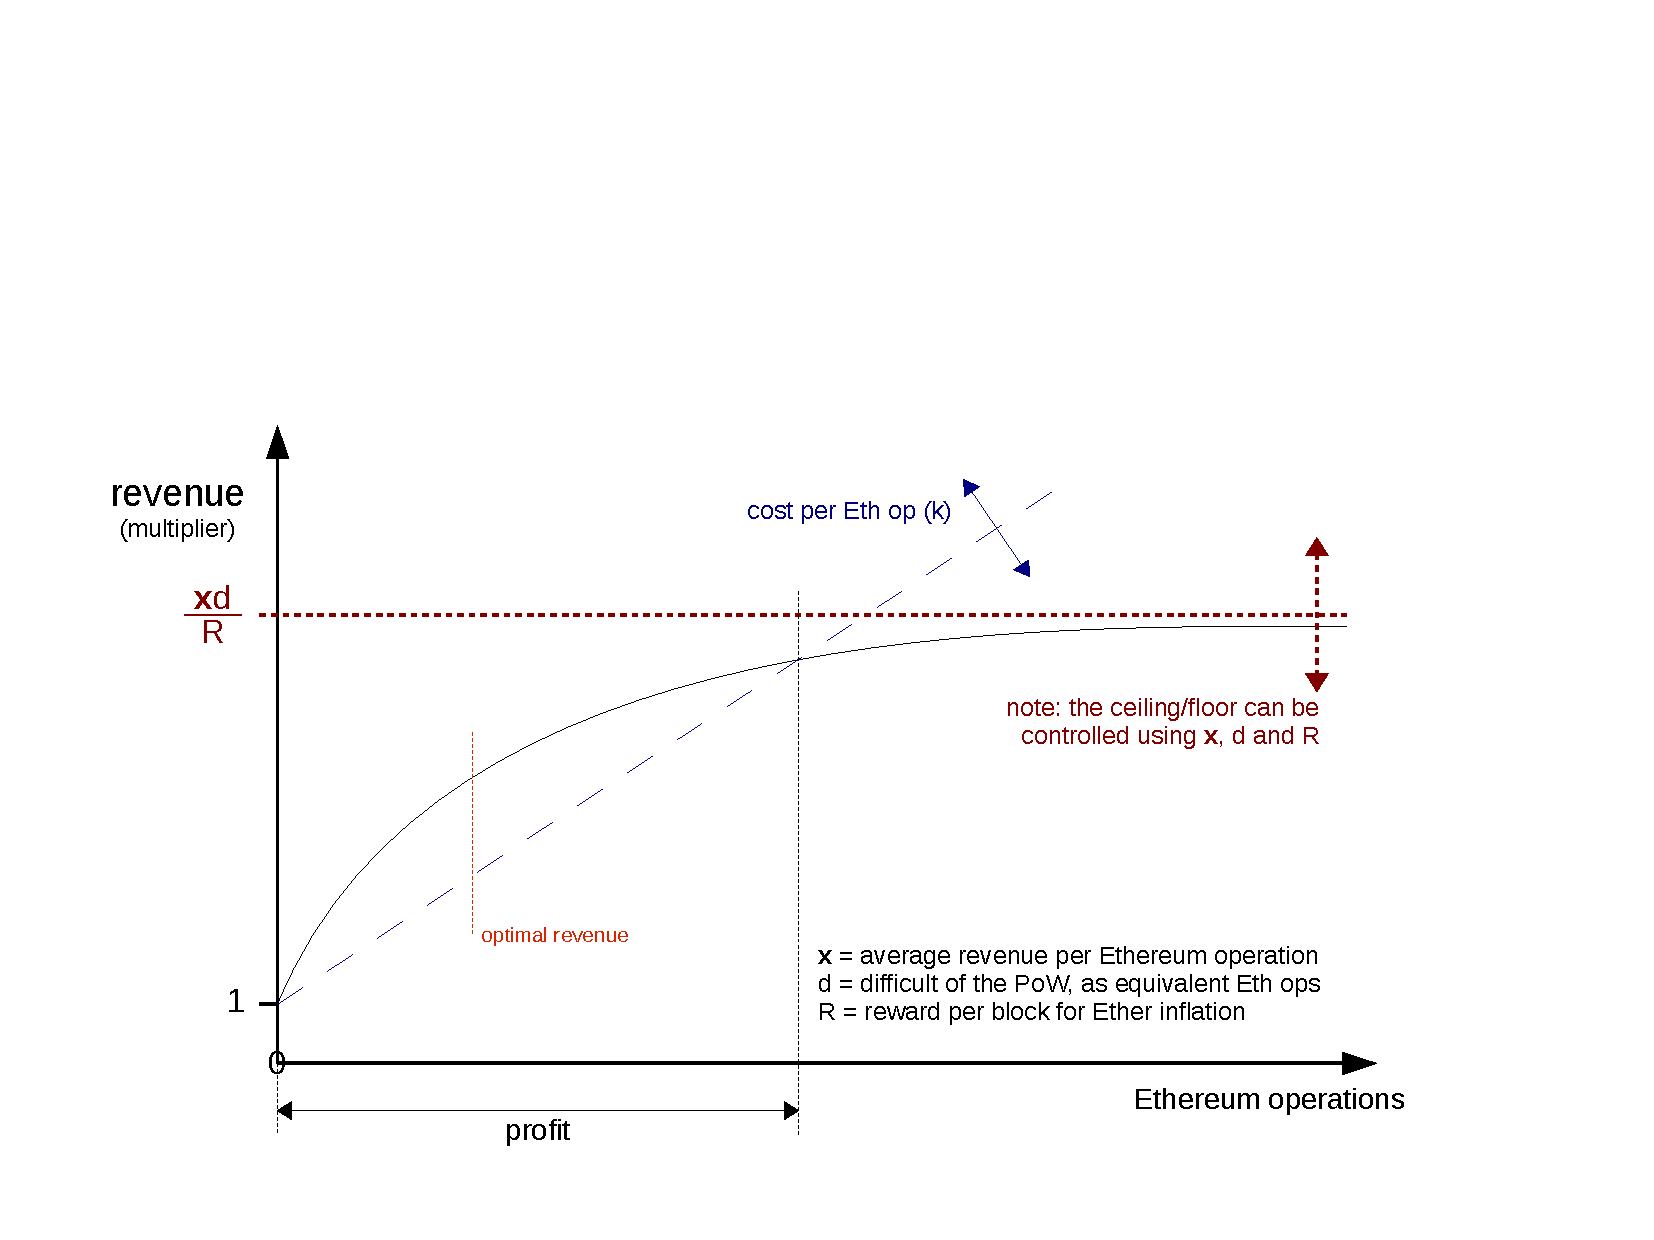
\includegraphics[trim=1cm 1cm 1cm 6cm, clip, width=15cm]{CompPayoff.pdf}
\end{center}

Two important notes regarding the generality of this result:
\begin{enumerate} \itemsep=0pt
\item This applies to any Ethereum computation level equilibrium: we just repeat the above analysis but consider everyone as doing some equal base level of transaction processing, and look at the extra transactions the node of interest is doing.
\item It doesn't matter where the ``revenue per operation'' comes from. If it is not from the basefee as built into Ethereum, it will be made up of ad-hoc payments that contracts offer to entice nodes to run them.
\end{enumerate}

Also note that if the $m\times$ node in question continues to do $r\times$ the PoW amount of effort in Ethereum computation, while all the other nodes will be continually subjected to a $r+1$ performance hit, so will the $m\times$ node when it goes for winning consecutive blocks, meaning that everyone's chances revert back to the original ratios for successive block attempts. In that case, the state update probabilities are:
\begin{align}
\mathrm{new\ state} &= 
\left(
\begin{matrix}
\mathrm{lose} & \mathrm{1^{st}win} & \mathrm{2^{nd}win}
\end{matrix}
\right)
\left(
\begin{matrix}
1 - p_1 & p_1 & 0 \\
1 - p_2 & 0 & p_2 \\
1 - p_1 & 0 & p_2 \\ 
\end{matrix}
\right) \\
\mathrm{steady\ state} &= 
\left(
\frac{1 - p_2}{1 + p_1 - p_2} \quad \frac{p_1(1-p_2)}{1 + p_1 - p_2} \quad \frac{p_1 p_2}{1 + p_1 - p_2}
\right) \\
\mathrm{with}\quad p_1 &= \frac{m}{(r+1)\N} \quad\mathrm{and}\quad p_2 = \frac{m}{\N}\\
\end{align}
so
\begin{align}
\mathrm{income} &= \frac{p_1}{1 + p_1 - p_2} ( r\x d + \R ) \\
 &= \frac{m(r\x d + \R)}{r\N + \N -mr} \\
 &= \left( \frac{(r\x d + \R)\N}{(\N(r+1)-mr)\R} \right) \frac{m\R}{\N} \\
 &\approx \left(\frac{r\x d + \R}{(r+1)\R}\right) \frac{m\R}{N} \quad \mathrm{when\ \N\gg m}
\end{align}
Hence, when the network is big enough, we can use the graph above.

Taking into account all the nodes, we can calculate the amount of Ethereum that will go into an average block...

However, a node could have such a low compute ability that the probability of getting a block on the block chain, and thus being able to be paid for the effort, is so low that it will never pay off. Having to continuously take hits from verifying transactions of other miners' winning blocks has the effect of lowering this threshold further, thus reducing Ethereum's total potential compute power. Is there anything to do about this? Nodes could simply not bother verifying winning blocks and hope that they are on the correct block chain, or they could maybe look to a trusted (set of) verifiers who could confirm, hopefully in a timely enough manner, that particular blocks are good. These are not desirable behaviours. Another question is whether excluding such nodes is actually bad thing at all: by having them add blocks to the block-chain, they will reduce the average Ethereum computation per block. This is a tempting argument, but is it balanced by the fact that having them as block verifiers is crucial to the stability and trustworthiness of Ethereum. Furthermore, there is a threshold below which a node would simply be too slow to even keep up with verifications. It is vital that this threshold remains low.

The above suggests that is advantageous to have low-power nodes work together, \ie merge to become a single node. However, if this happens on too large a scale we move towards de facto centralization, which is bad. Ideally, we want nodes to merge only if they are small. We would like to see the attractiveness of merging being (vaguely) inversely proportional to size. Calculations are needed for bitcoin, but so far that seems to be working OK.

I am ignoring, here, all participants who are just verifying the block chain and not taking part in mining, perhaps because their computer has no chance of winning the PoW race. There is nothing to be done about this because there is no practical way of getting any sort of incentive to them beyond the ability to participate in Ethereum and be assured of its legitimacy. However, one of the aims of Ethereum is to maximize the number of people who can be miners. Many people will simply choose to rely of others to verify everything for them. They all remain outside the system and therefore outside this analysis.

\subsection*{Final Thoughts}

Still looking...


\end{document}